\chapter{Mobiles Ad Hoc Routing}
Mobile ad hoc Netze sind drahtlose Netzwerke, die sich schnell und konfigurationslos einrichten lassen.
Sie müssen in der Lage sein, eigenständig Verbindungen aufzubauen, ohne sich dabei auf eine vorkonfigurierte
Infrastruktur zu stützen.
Beispielsweise zur Kommunikation zwischen Fahrzeugen oder zum Aufbau einer Notfallinfrastruktur bei Katastrophen
werden mobile und dynamische Netzwerke zur Koordinierung eingesetzt.

Chien-Chung Shen und Chaiporn Jaikaeo 
%\cite{shen_ad_2005}
implementieren mittels Schwarmintelligenz ein reaktives Multicast Routingprotokoll,
welches Routingpfade durch probabilistische Erkundungsstrategien optimiert, die an das Verhalten von Ameisen angelehnt sind.

Bisherige Ansätze, die Baumstrukturen verwenden, um Multicastnachrichten zu versenden,
sind sehr anfällig für Ausfälle von Zwischenknoten, da es meistens nur einen einzigen Pfad zwischen Sendern und Empfängern gibt.
Die Alternative ist ein Gitterkonstrukt mit mehreren Pfaden von Sender zu Empfänger

Das Protokoll \emph{Multicast for Ad Hoc Networks with Swarm Intelligence}, kurz \emph{MANSI}, benutzt diesen Ansatz.
Es wird im nächsten Kapitel genauer erläutert.

\section{MANSI}
MANSI ist ein Multicastprotokoll für mobile ad hoc Netzwerke.
Grundlage des Protokolls ist die Reduzierung der Anzahl von Zwischenknoten (Hops), einer multicast Verbindung.
Dafür werden bestimmte Kontrollpakete  versendet, die Metaformationen über das Netzwerk an Knoten verteilen, ähnlich wie Ameisen, die Pheromonspuhren auf ihren Wegstrecken zurück lassen.

Durch die Art der indirekten Kommunikation\footnote{Diese Form der Kommunikation wird auch als
\emph{Stigmergie} bezeichnet.} optimieren sich die Routingpfade nach und nach von selbst.

Bei der multicast Übertragung werden Nachrichten an eine Gruppe von Teilnehmern (Knoten) gesendet.
In MANSI hat jede Gruppe dabei einen zentralen Kernknoten.
Dieser kann entweder ein Empfängerknoten aus der Gruppe oder ein Sender sein.

Außerdem werden Zwischenknoten bestimmt, die zusammen ein sogennantes \emph{forwarding set} bilden,
das alle Knoten der Gruppe verbindet.
Die Knoten des forwarding sets sind dabei nicht Mitglieder der Gruppe und bestehen 
anfangs aus dem kürzesten Pfad zwischen Kern und Knoten der Gruppe.
Sie dienen lediglich der Weiterleitung von Nachrichten an Knoten der Gruppe.

Während einer Multicastsitzung entwickelt sich dieses forwarding set mittels Schwarmintelligenz weiter, sodass 
eine möglichst geringe Anzahl an Zwischenknoten erreicht wird.

Der Kernknoten ist, anders als beim \emph{core-based tree protocol}
%\cite{ballardie_core_1993}
nicht statisch, sondern wird bei jeder Multicastsitzung neu bestimmt.
Genauer gesagt wird der erste aktive Knoten Kern einer Gruppe.
Dafür sendet er ein \textsc{core announce} Paket an alle Teilnehmer des Netzwerks.
Jeder Teilnehmer sendet dann ein \textsc{join request} zurück an den Kern.
Jeder Kern, der ein \textsc{join request} an sich selbst empfängt, wird Zwischenknoten der Gruppe.

Damit neue Knoten den Kern kennen, muss dieser periodisch das Netz mit \textsc{core announce} Paketen fluten,
solange eine Multicastsitzung besteht.

\section{Verbesserung durch Schwarmintelligenz}
Die Verbesserung des forwarding sets geschieht, indem jeder Teilnehmer periodisch \textsc{forward ant} Pakete an Nachbarknoten sendet,
die opportunistisch neue Routen erkunden, in der Hoffnung eine bessere Gesamtroute zu finden.
Der Prozess ist in Abbildung \ref{fig:MANSI1} veranschaulicht:
(a) zeigt den initialen Pfad des forwarding sets.\\
(b) zeigt den verbesserten Pfad durch Schwarmintelligenz.


\begin{center}
\begin{figure}[htbp]
 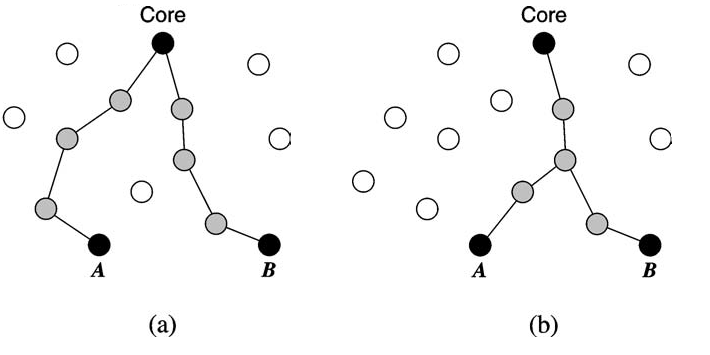
\includegraphics[width=12cm,keepaspectratio=true]{./images/adhoc.png}
 \caption{Beispielskizze einer Multicastverbinung von drei Gruppenmitgliedern}
\label{fig:MANSI1}
\end{figure}
\end{center}

Erreicht ein \textsc{forward ant} Paket einen Knoten, der selbst forwarding Knoten der Gruppe ist,
wird er zu einer \textsc{backward ant} und geht zurück an seinen Absender.
Bei jedem Zwischenknoten, der dabei genutzt wird,
berechnet das Netzwerk die Kosten, den aktuellen Knoten zum forwarding set hinzuzufügen.
Außerdem wird der ``Pheromongehalt'' 
des Knotens berechnet. Dieser ist umgekehrt proportional zu den Kosten.
Die Informationen werden dann lokal im Knoten gespeichert.

Nachfolgende \textsc{forward ants} entscheiden dann anhand des Pheromongehalts des Knotens, welchen Weg sie weiter gehen werden.

In Abbildung \ref{fig:MANSI2} wird der Updateprozess illustriert.
Sobald eine \textsc{forward ant} den Knoten D erreicht hat, wird sie zur \textsc{backward ant} und geht über C 
zurück nach A.
Die Kosten, dass C in das forward set integriert wird, beträgt Null,
da C direkt benachbart mit D ist.
Nun wird über den Pheromongehalt der Knoten entschieden, welche Route die Pakete nehmen.
C hat in dem Fall den höchsten Anteil, was dazu führt ,dass die Knoten E, F und G vom forwarding set entfernt werden.

\begin{center}
\begin{figure}[htbp]
 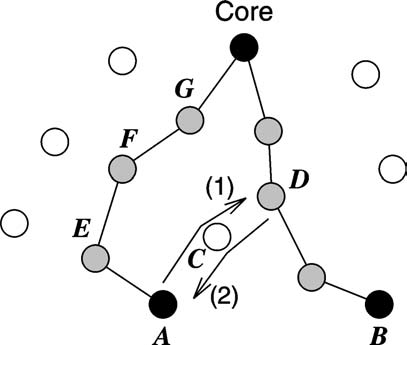
\includegraphics[width=10cm,keepaspectratio=true]{./images/adhoc2.png}
 \caption{Verbesserung der Route durch forward und backward ants}
\label{fig:MANSI2}
\end{figure}
\end{center}


\section{Ameisen Todes-Spirale}
Bei Ameisenkolonien ist ein seltenes Phänomen zu beobachten:
Ameisen folgen immer der Ameise, die direkt vor ihnen läuft, um ans Ziel zu kommen, außer natürlich die Vorderste.
Sie folgt einer Pheromonspur oder erkundet das Gebiet zufällig.

Gelegentlich kommt es jedoch vor, dass die vorderste Ameise irgendwie einem ihr Folgenden hinterher läuft
Dann drehen sich die Ameisen im Kreis, bis der gesamte Ameisenzug verhungert.
Dieses Phänomen wird als \emph{Ameisen Todes-Spirale}, oder \emph{ant mill}, bezeichnet.
%\cite{schneirla_unique_1944}
Übertragen auf das Routing muss also darauf geachtet werden, dass im Routinggraph keine Zyklen entstehen und er komplett vom Kern abgekoppelt wird.
Dies kann passieren, wenn eine \textsc{forwarding ant} den eigenen Pfad zum Set hinzufügt.
Verhindert werden kann dies, indem jeder Knoten eines Sets einen \emph{Höhenwert} und eine \emph{ID} besitzt.
Dieser Höhenwert $h$ errechnet sich aus dem Maximum aller IDs, die den selben Pfad zum Kern benutzen.
Der Kern selbst hat die Höhe $\infty$.
Eine \textsc{forward ant} $a$ wird nur dann zu einer \textsc{backward ant}, wenn sie auf einen forward Knoten trifft, der einen höheres $h$ 
hat, als die ID des Ursprungsknoten von $a$.
Dadurch werden Zyklen verhindert, die sich vom Kernknoten abkoppeln, gleichzeitig gedoch auch die Dynamik des Netzwerks eingeschränkt.
Es ist daher nicht garantiert, dass für die Zeit $t: t \rightarrow \infty$ das Netz Optimal wird.

Durch das Prinzip der Pheromonspuhren und Erkundungsameisen wird das Protokoll von sich aus für mobile Szenarien geeignet.
Werden Knoten aus den Netzwerk entfernt, passt sich das forwarding set einfach an, indem neue Wege erkundet werden.
Abgebrochene Verbindungen werden im günstigsten Fall automatisch überbrückt, wenn ein alternativer Pfad bevorzugt wird, der zuvor nicht benutzt wurde, 
weil er einen geringeren Pheromonwert hatte. 
In mobilen Netzen können sich außerdem die optimalen Routingwege ändern, dies wird durch die probabilistische Natur der \textsc{forward ants} bewältigt.
Sie erkunden und bewerten periodisch neue Wege.

Bei dünn besiedelten Netzwerken können gerade in mobilen Szenarien instabile Netze entstehen.
In MANSI wird dies über einen Stabilitätsindexes verbessert.
Jeder Knoten hält die \emph{normalized link failure frequency},
also die Verbindungsfehlerrate.
Diese gibt Aufschluss über die relative Stabilität naheliegender Knoten und es können instabile Bereiche im Netzt vom Routing ausgeschlossen werden.

\section{Fazit}
Shen und Jaikaeo haben mit MANSI ein alternatives Multicast Routingprotokoll entwickelt, das sich für mobile ad hoc Netze eignet.
Das Netzwerk benutzt ein Kernbasierten Ansatz, der durch Zwischenknoten und forwarding sets ein stabiles und dynamisches Gitterkonstrukt aufbaut,
welches mittels Schwarmintelligenz verbessert wird.
Mobilität und Dynamik wird durch diese Routingstrategie automatisch gewährleistet.
In den Bereichen Load Balancing, Energieerhaltung und Sicherheit bietet das Protokoll Verbesserungspotential.

